\chapter{System Architecture}
\section{Data Warehouse Architecture}
The system follows a Kimball bottom-up design: raw extracts are staged in Snowflake \texttt{RAW}, the conformed dimensions and facts are deployed to Snowflake \texttt{MART}, and the analytics layer and Streamlit dashboard consume them. The stages are:

\begin{enumerate}
    \item \textbf{Source Systems:} The six raw CSV files of the PKDD dataset (clients, accounts, dispositions, transactions, loans, and district demographics).
    \item \textbf{Staging:} The \texttt{RAW} schema in Snowflake holds five untouched extracts with source row counts; the district file is used to derive branch labels.
    \item \textbf{Data Warehouse:} The \texttt{MART} schema holds the five conformed dimensions, the two fact tables, the analytics tables, and the reporting views.
    \item \textbf{Analytics Layer:} A leakage-safe feature mart, trained model scores, association rules, and cluster labels are written back to \texttt{MART}.
    \item \textbf{Presentation:} A Streamlit application reads the modelled tables and saved artifacts to render eight interactive review pages.
\end{enumerate}

\begin{figure}[H]
    \centering
    \resizebox{\textwidth}{!}{
    \begin{tikzpicture}[
        node distance=3.5cm,
        every node/.style={font=\sffamily},
        % Standard box
        box/.style={rectangle, draw=midgray!50, thick, fill=white, minimum width=3.5cm, minimum height=1.6cm, align=center, rounded corners=6pt},
        % Database cylinder
        db/.style={cylinder, draw=midgray!50, thick, fill=white, shape border rotate=90, aspect=0.25, minimum width=3.5cm, minimum height=2.8cm, align=center, inner sep=5pt},
        % Arrow style
        arrow/.style={-{Stealth[scale=1.2]}, very thick, color=midgray},
        % Label style
        lbl/.style={above, yshift=2pt, font=\small\sffamily, color=midgray!90!black}
    ]
        
        \node[box, fill=tablebg] (source) {
            \textbf{\textcolor{midgray!90!black}{Source Data}}\\[2pt]
            \small(PKDD CSV extracts)
        };
        
        \node[db, fill=tablebg, right=of source] (raw) {
            \vspace{0.3cm}\\
            \textbf{\textcolor{accent}{Snowflake RAW}}\\[2pt]
            \small(staging tables)
        };
        
        \node[db, fill=tablebg, right=of raw] (mart) {
            \vspace{0.3cm}\\
            \textbf{\textcolor{primary}{Snowflake MART}}\\[2pt]
            \small(galaxy + analytics)
        };
        
        \node[box, fill=tablebg, right=of mart] (bi) {
            \textbf{\textcolor{secondary}{Streamlit}}\\[2pt]
            \small(review dashboard)
        };
        
        \draw[arrow] (source) -- node[lbl] {Extract \& Load} (raw);
        \draw[arrow] (raw) -- node[lbl] {Transform} (mart);
        \draw[arrow] (mart) -- node[lbl] {Read} (bi);
        
    \end{tikzpicture}
    }
    \caption{Bottom-up warehouse architecture on Snowflake with a Streamlit presentation layer}
    \label{fig:architecture}
\end{figure}

The full pipeline is expanded in Figure~\ref{fig:system_arch}. Five source extracts are staged in \texttt{RAW}; the district file is used to label branches. The conformed dimensions and two fact tables are deployed to \texttt{MART}, followed by the leakage-safe analytics tables, and the Streamlit dashboard reads those modelled tables directly. No reporting tool sits between the warehouse and the browser.

\begin{figure}[H]
    \centering
    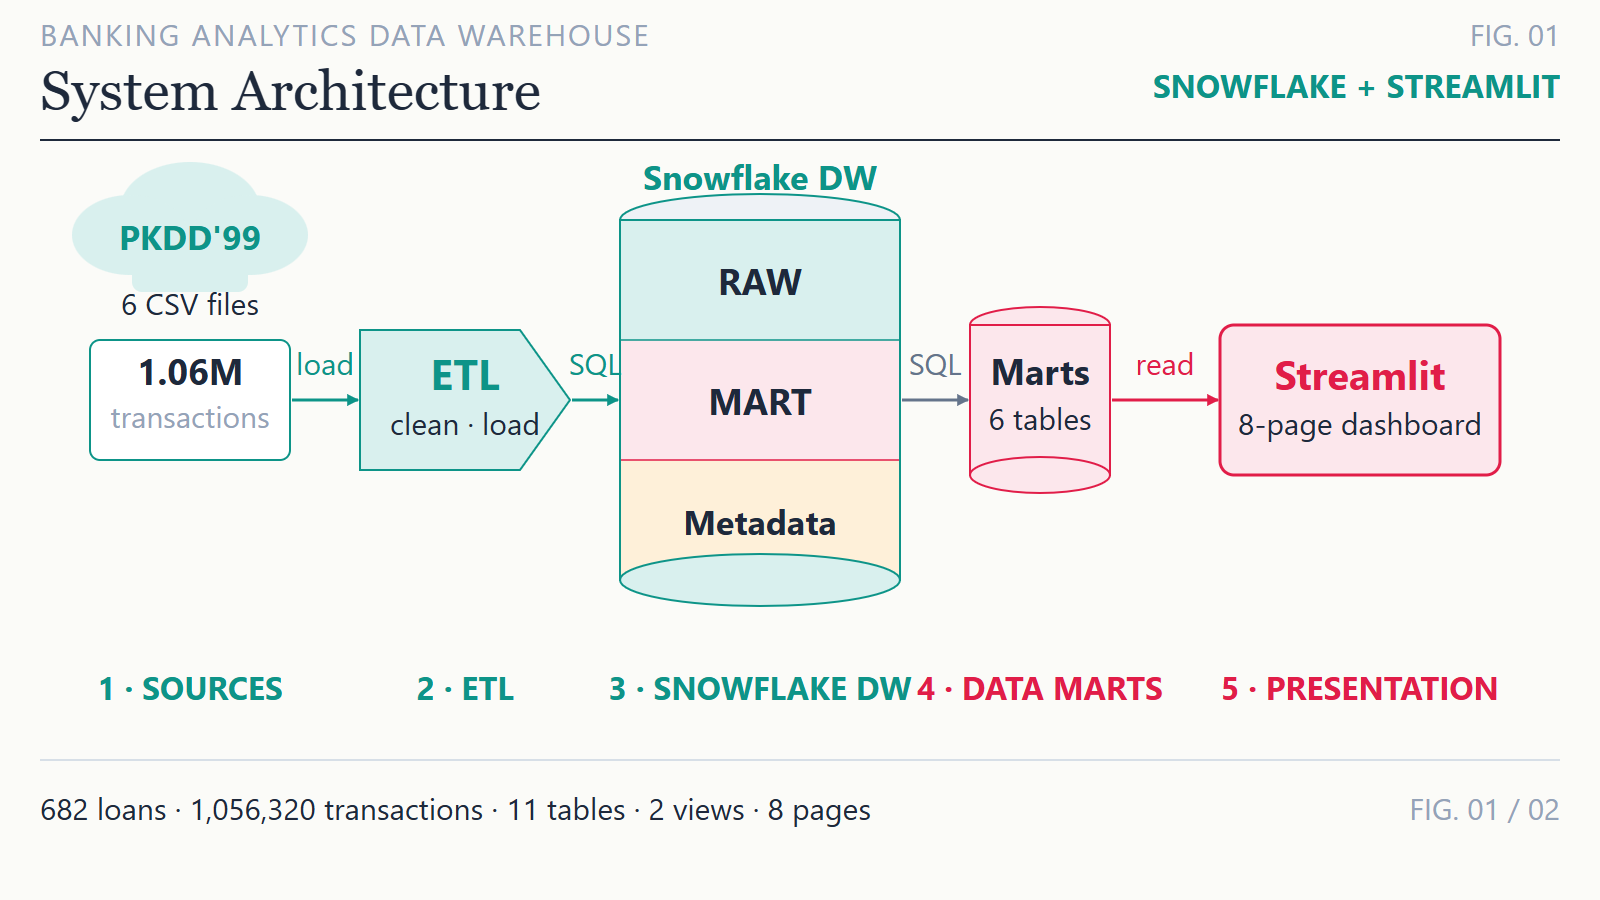
\includegraphics[width=0.95\textwidth]{figures/01_system_architecture.png}
    \caption{End-to-end Snowflake pipeline from raw extracts to the Streamlit review dashboard}
    \label{fig:system_arch}
\end{figure}

\begin{figure}[H]
    \centering
    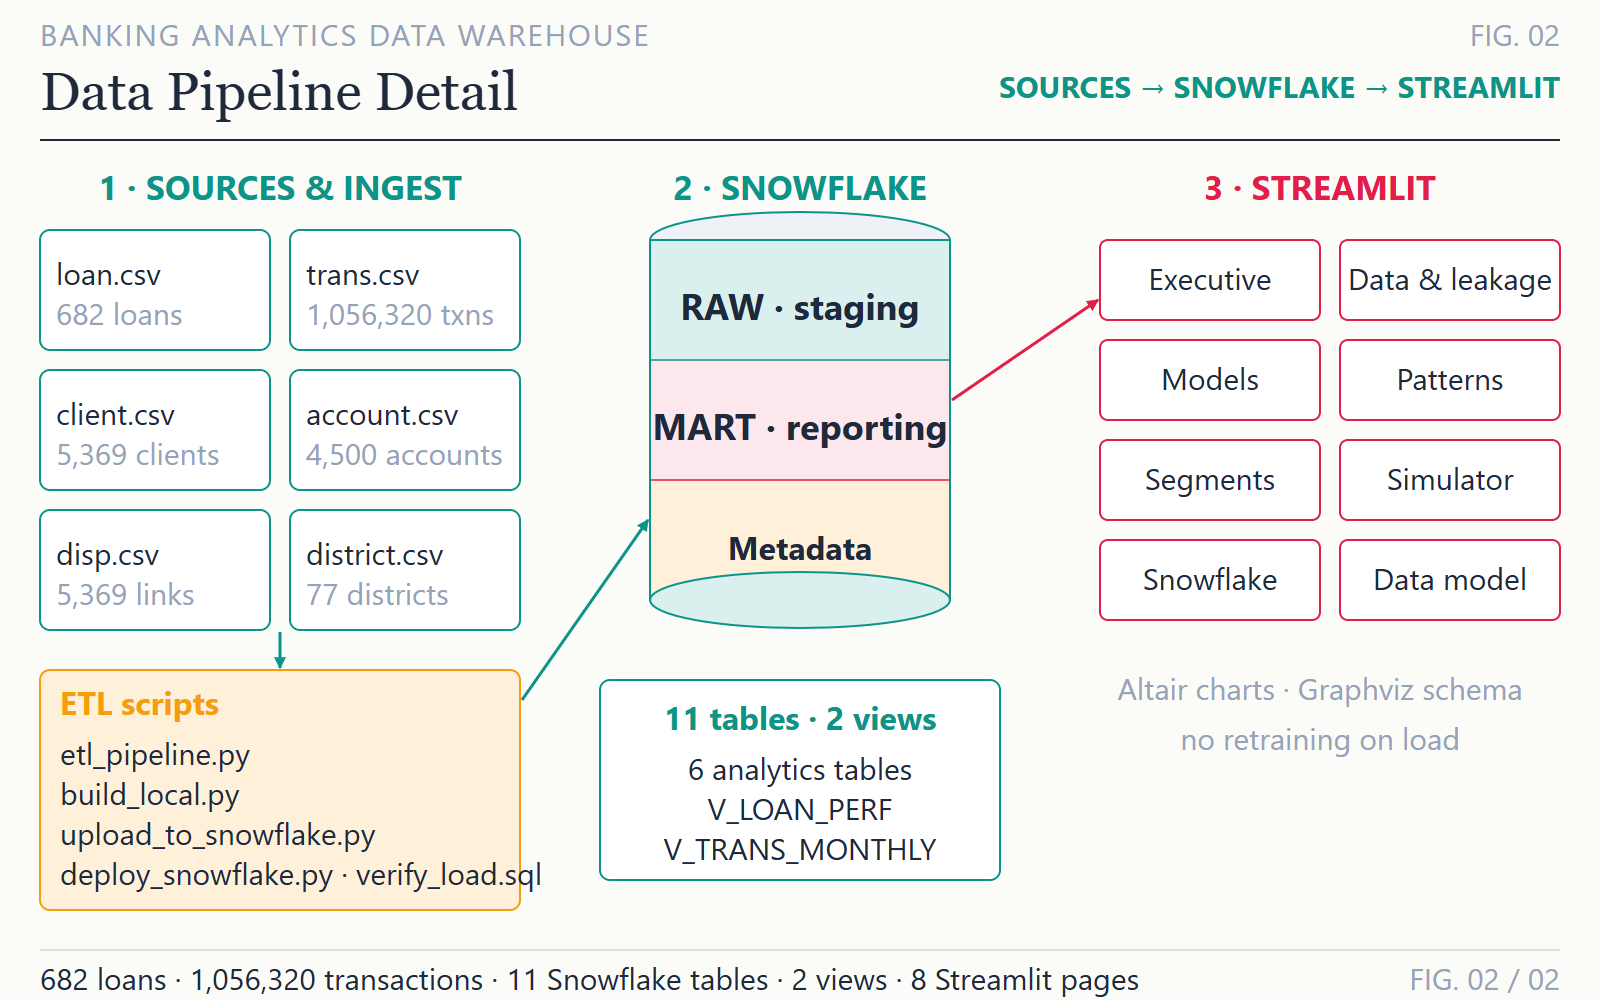
\includegraphics[width=0.95\textwidth]{figures/02_data_pipeline.png}
    \caption{Pipeline detail: the six source extracts, the ETL scripts, the Snowflake RAW and MART layers, and the eight Streamlit pages}
    \label{fig:pipeline_detail}
\end{figure}

\section{Requirement Analysis}
The following requirements drove the design:
\begin{itemize}
    \item \textbf{Data Integration:} Extract the historical banking data, stage it without modification, and load a central modelled repository with repeatable scripts.
    \item \textbf{Dimensional Modelling:} Support slicing across time, geography (district/branch), and customer demographics through conformed dimensions.
    \item \textbf{Metric Calculation:} Produce loan default rates, balance-derived behaviour measures, and segment summaries from the same warehouse.
    \item \textbf{Leakage Control:} Every predictive feature must be computed from pre-loan transactions only, and the condition must be verified automatically.
    \item \textbf{Review Support:} Expose scores, rules, and segment labels through an interactive dashboard rather than a static report.
\end{itemize}

\section{Technology Stack}
The implementation uses Python and pandas for extraction and transformation, Snowflake for the warehouse, scikit-learn for classification and clustering, mlxtend for Apriori and FP-Growth, Altair and Graphviz for dashboard visuals, and Streamlit for the application layer. Loader scripts create or replace objects and truncate target tables before writing, so a rerun does not append duplicate rows.

\section{ETL Validation and Data Integrity}
The transformation stage handles null values, parses date strings into standard date keys, generates surrogate identifiers, and casts financial amounts to numeric types. To prove that no records are lost during extraction and load, row counts are reconciled between the source files and the loaded warehouse tables.

\begin{table}[H]
    \centering
    \begin{tabular}{|l|c|c|c|}
        \hline
        \textbf{Entity} & \textbf{Raw CSV Rows} & \textbf{Loaded DB Rows} & \textbf{Accuracy Match} \\
        \hline
        Transactions & 1,056,320 & 1,056,320 & 100\% \\
        Loans & 682 & 682 & 100\% \\
        Accounts & 4,500 & 4,500 & 100\% \\
        Customers & 5,369 & 5,369 & 100\% \\
        \hline
    \end{tabular}
    \caption{ETL data reconciliation and accuracy proof}
    \label{tab:etl_accuracy}
\end{table}

Referential integrity is enforced by checks that each fact row resolves to a valid dimension key. The build also verifies that the number of feature rows equals the number of loan facts, and that no feature row contains post-loan transaction activity.
